% 
% Annual Cognitive Science Conference
% Sample LaTeX Paper -- Proceedings Format
% 

% Original : Ashwin Ram (ashwin@cc.gatech.edu)       04/01/1994
% Modified : Johanna Moore (jmoore@cs.pitt.edu)      03/17/1995
% Modified : David Noelle (noelle@ucsd.edu)          03/15/1996
% Modified : Pat Langley (langley@cs.stanford.edu)   01/26/1997
% Latex2e corrections by Ramin Charles Nakisa        01/28/1997 
% Modified : Tina Eliassi-Rad (eliassi@cs.wisc.edu)  01/31/1998
% Modified : Trisha Yannuzzi (trisha@ircs.upenn.edu) 12/28/1999 (in process)
% Modified : Mary Ellen Foster (M.E.Foster@ed.ac.uk) 12/11/2000
% Modified : Ken Forbus                              01/23/2004
% Modified : Eli M. Silk (esilk@pitt.edu)            05/24/2005
% Modified : Niels Taatgen (taatgen@cmu.edu)         10/24/2006
% Modified : David Noelle (dnoelle@ucmerced.edu)     11/19/2014
% Modified : Roger Levy (rplevy@mit.edu)     12/31/2018



%% Change "letterpaper" in the following line to "a4paper" if you must.

\documentclass[10pt,letterpaper]{article}
\usepackage{cogsci}
\usepackage{dsfont}
\usepackage{bm}
\usepackage{amssymb}
\usepackage{indentfirst}
\usepackage{graphicx}
\usepackage{subfig}
\usepackage{multirow}

%\cogscifinalcopy % Uncomment this line for the final submission 


\usepackage{pslatex}
\usepackage{apacite}
\usepackage{float} % Roger Levy added this and changed figure/table
                   % placement to [H] for conformity to Word template,
                   % though floating tables and figures to top is
                   % still generally recommended!

%\usepackage[none]{hyphenat} % Sometimes it can be useful to turn off
%hyphenation for purposes such as spell checking of the resulting
%PDF.  Uncomment this block to turn off hyphenation.


%\setlength\titlebox{4.5cm}
% You can expand the titlebox if you need extra space
% to show all the authors. Please do not make the titlebox
% smaller than 4.5cm (the original size).
%%If you do, we reserve the right to require you to change it back in
%%the camera-ready version, which could interfere with the timely
%%appearance of your paper in the Proceedings.



\title{How to Make a Proceedings Paper Submission}
 
\author{{\large \bf Morton Ann Gernsbacher (MAG@Macc.Wisc.Edu)} \\
  Department of Psychology, 1202 W. Johnson Street \\
  Madison, WI 53706 USA
  \AND {\large \bf Sharon J.~Derry (SDJ@Macc.Wisc.Edu)} \\
  Department of Educational Psychology, 1025 W. Johnson Street \\
  Madison, WI 53706 USA}


\begin{document}

\maketitle


\begin{abstract}

\textbf{Keywords:} 
\end{abstract}


\section{Introduction}

Identifying the causes of an event is a very important ability that people largely rely on in common life. Even if reasonning about causes doesn't generally pose problems and comes up with clear answers about what caused an event, it is sometimes much more difficult to disambiguous an event and answer such a question. When divergent causal intuitions are involved it can be hard to decide for one candidate cause rather than an other. This can lead to very different and serious implications, especially legal ones. For example a well-known story in the literature is the ``Irish case'', a real-world example of a court case: [include here Irish case]. In such legal contexts determining the main causes of an event is an extremely important task that involves finding who or what is at fault in dramatic accidents, property damage, etc. and can pose a veritable challenge. Here massive fines, jail sentences or death penalties can be the outcomes of the inferred causal history of an event. Reasonning about causes, however, is often implied in much more naive and common circonstances and doesn't necessary pose any difficulty --e.g. identifying what is the cause of the bottle shattering. But even in very simple situations like that, it is sometimes not so easy to theoretically explain and predict intuitive responses that people give. [Include here Susy vs Bob example]. In all these common-life situations we want to know what the \textit{actual cause} of an event is, in a specific context. That is we don't want here to infer some general causal laws responsible for the occurrence of an event but understand what is the main or most intuive singular causes in particular cases. The current paper focuses on causal judgements of the latter type, that is on the concept of \textit{actual} and not \textit{general} causation\footnote{also called ``token'' or ``singular'' causation}, following a distinction that has been frequently made in the litterature. Causal judgements have been widely studied and there are existing models of actual causation that aim to capture people's inferences about the causes of a single event. Current research on actual causation mainly relies on two different interpretations of causality : the counterfactual account (CF) or the physical process one (PP).

\begin{figure}[ht]
\begin{center}
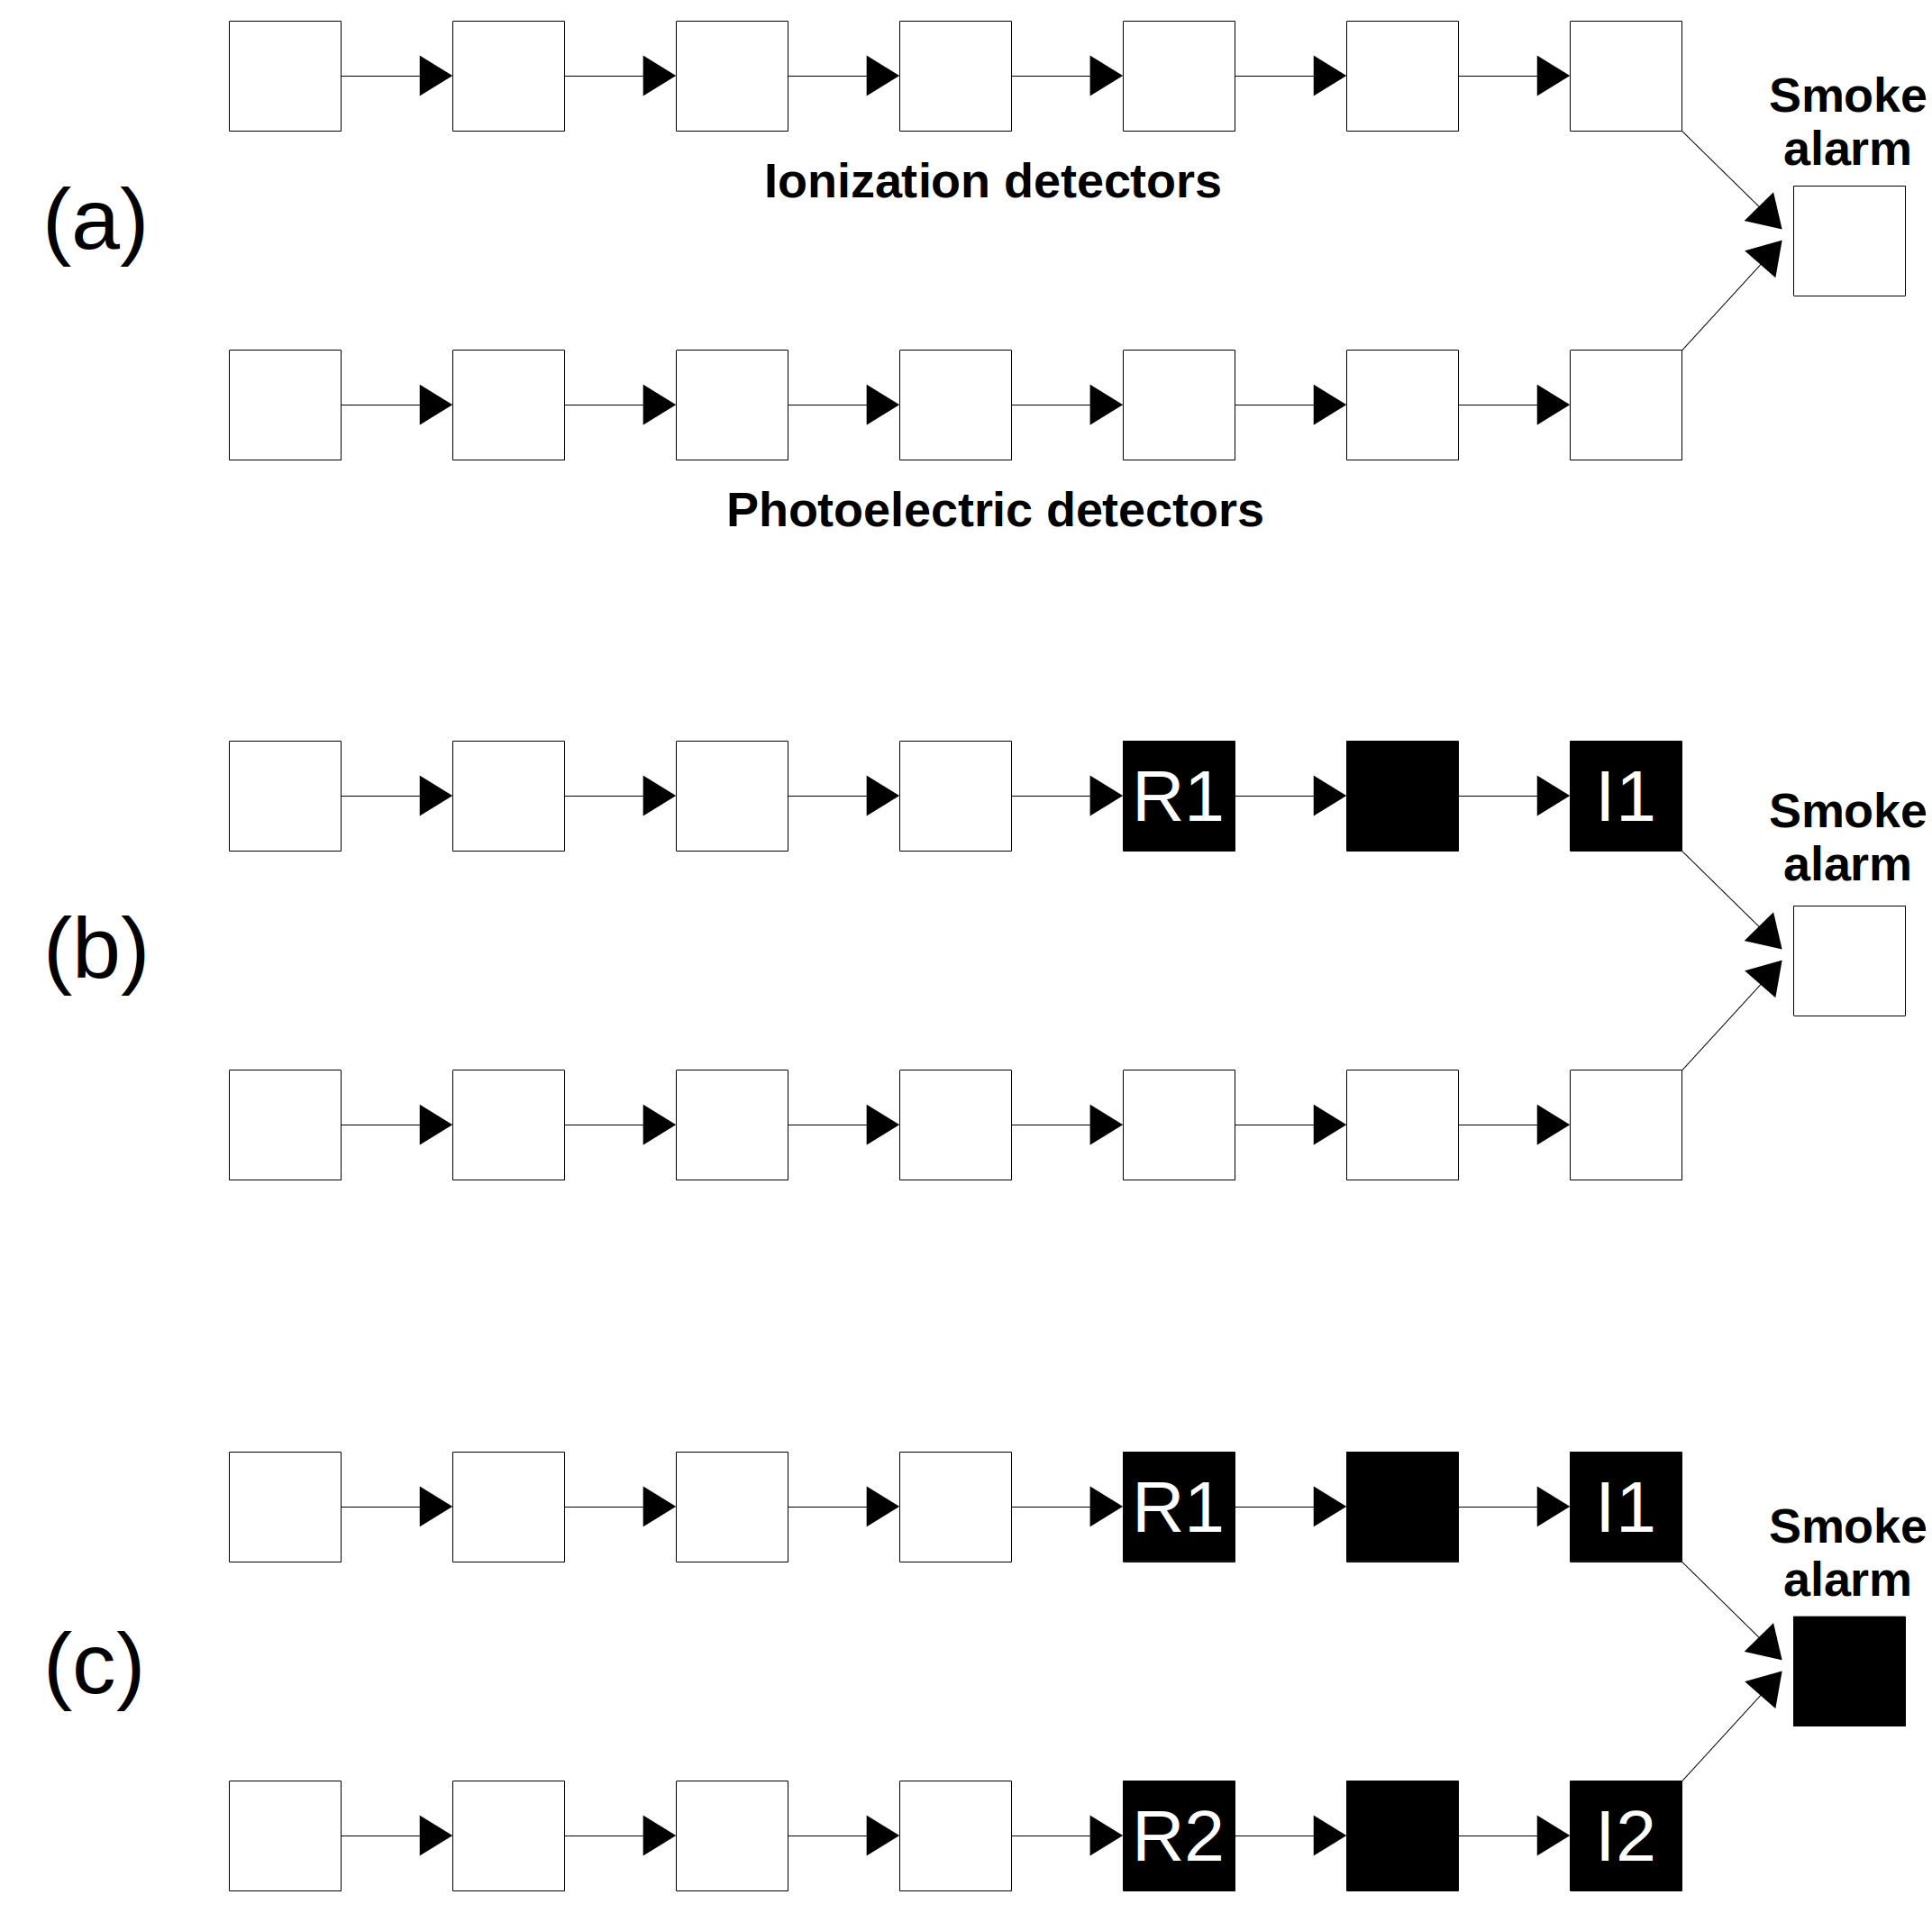
\includegraphics[width=6cm]{intro}
\end{center}
\caption{This is a figure.} 
\label{fig:1}
\end{figure}

According to the first interpretation, the general idea is that an event A is said to be a cause of a distinct event B if the occurrence of A makes a difference in the occurrence of B. In other words if B would have been different without A, then A is an actual cause. More precisely A is a cause of B if and only if A and B are true, and A hadn't occurred B wouldn't have occurred. [Example of Suzy only] This type of explanation calls upon counterfactual scenario or possible worlds where the presumed cause of the effect is removed from the system while all other relevant factors are kept as unchanged as possible compared to the actual world. However, a first well-known challenge that the CF account encounters is that it is not clear which counterfactual world we have to take into account in order to justify a singular cause, and how to accurately compare those counterfactuals. Again let's say that Suzy throws a rock at a bottle but this time Bob as well throws a rock at the same bottle with the same precision as Suzy. Suzy's rock reaches the bottle just a second before Bob's and breaks it. According to the CF account if Suzy hadn't thrown the rock, the bottle would have still shattered since Bob's rock would have hit it regardless. So following the general idea mentionned above, Suzy's throw cannot be the cause of the bottle shattering -- which is counter-intuitive. This is an example of a general type of cases we call \textit{late preemption} and refers to the fact that the final event -- i.e. the effect -- is ``overdetermined'' [Hall]. A first common attempt to face the problem is to say that the bottle-shattering event that results from Suzy's throw is qualitatively different from the the bottle-shattering event that follows from Bob's throw. In other words A is a cause of B if and only if A and B occur, and A hadn't occurred B wouldn't have occurred at all or would have been delayed. Thus Suzy's throw is indeed the cause of the bottle-shattering event that occurs at the time it did. 

[Halpern and Pearl solution : graphical models, static, pb of modelling, without time, etc.] 
[Then, more general problem with counterfactual dependance].

The physical process account of causation gives a completely different interpretation of causality and states that an event A causes B when there is a physical connection between them. Several theories have been proposed to caracterise this physical connection. In one of its latest and probably most convincing formulation, we have to distinguish two things : causal process and causation or causal interaction. A causal process is a physical process involving an object which conserves a certain quantity accross space and time. The conserved quantity is typically a measurable physical property of the object like the mass-energy, etc. and is precisely what scientific theories are meant to formalize. In that sence both Suzy's and Bob's throw are causal processes. A causal interaction or causation is an exchange of that conserved quantity, for example the mass-energy of the rock to the glass of the bottle. According to this definition, only Suzy's throw involves a causal interaction with the bottle. However the PP account of causation doesn't consider as genuine causation some very common cases that people intuitively judge as proper example of causation. For example if I hold the head of my ennemy under water and make him die, I'm not genuinely the cause of his death; rather I'm actually preventing the possibility of a genuine causation which is the physical process of breathing oxygen in order to live. The main problem is that, as a consequence, the PP account not only goes sometimes against some of our best causal intuitions, but also needs the counterfactual analysis as well to ground cases of \textit{quasi-causation} by omission or prevention like the latter one.


[?? A third account : probability raising ??]


\section{Theoretical proposition}

As a result of the preceeding analysis it seems that none of the current main theories of actual causation gives a satisfying explanation of the causal judgements that people actually do. This paper aims at solving the problem by interpreting causality in a completely different way. In the CF framework events are represented as mere propostions and causation is thought as a relation between static states. The PP account is meant to give an epistemological definition of the concept of causation and not an explanation of how people actually rely on temporal informations to make causal judgements. By contrast this paper focuses on the role of temporal information for inferring causal relationship between events qua changes of states over time. In other words we hypothesised that people's causal judgements are influenced by not only the values of all relevant variables at the time the effect occurs, but also the temporal order in which these variables took their values. [?? Add a concrete example ??] This approach has some precedent in the literature but has not been developed carefully and has never been tested experimentally as we intend to do. We add further that people mainly identify causation with a \textit{continuous} sequence of changes of states over time. The underlying intuition is that people trace back the history of changes from the immediate one that directly brought about the occurrence of the effect, up to the root change in the system that initiated the series of changes along the path. As we think that in common life it is really rare to see simultaneously two or more events occurring at the very same time and producing some common effect, we also want to postulate a \textit{no coincidence principle}. Relying on this principle we can split the system's time frame in units of time that are small enough to have no more than one event\footnote{Again we insist on the definition of \textit{event} as \textit{change of state}.} per unit. Lets represent by $\mu^{\emptyset}_{z_{i\rightarrow j}}(t)$ a change of state at time $t$, from variable $Z=z_i$ to $Z=z_j$, $\forall i,j\in \mathds{R}_+$. Here $Z$ is the variable we want to reason about and has no children (represented by the empty set $\{\emptyset\}$). Formalizing our above mentioned idea we first have to find $\mathcal{U}^Z_{\bm{y}_{i\rightarrow j}}(t-1)$, that is the set of the immediate changes in the parents $\bm{Y}$ of the variable $Z$ at time $t-1$ that led to the observed change in $Z$ at time $t$. So we want to find $\mathcal{U}$ such that $\mathcal{U}^Z_{\bm{y}_{i\rightarrow j}}(t-1)\rightarrow \mu^{\emptyset}_{z_{i\rightarrow j}}(t)$. According to our \textit{no coincidence principle} $\mathcal{U}$ is either empty or a singleton -- including only one parent whose value changed. Lets say that at $t-1$ we find a change in a parent variable $Y$, so $\mathcal{U}^Z_{\bm{y}_{i\rightarrow j}}(t-1)=\{\mu^{Z}_{y_{i\rightarrow j}}(t-1)\}$. Then we want to find the set of changes such that $\mathcal{U}^Y_{\bm{x}_{i\rightarrow j}}(t-2)\rightarrow \mu^{Z}_{y_{i\rightarrow j}}(t-1)$, that is the set of immediate previous changes in the parents $\bm{X}$ of the variable $Y$ at time $t-2$ that led to the observed change in $Y$ at time $t-1$. Following the same logic we suggest that if $\mathcal{U}^X_{\bm{w}_{i\rightarrow j}}(t-3)\rightarrow \mu^{Y}_{x_{i\rightarrow j}}(t-2)$ is such that $\mathcal{U}^X_{\bm{w}_{i\rightarrow j}}(t-3)=\emptyset$, then it means that $\mu^{Y}_{x_{i\rightarrow j}}(t-2)$ represents the chronologically first change along the path, occurring in $X$, and we suggest that this change is identified as being the main cause of $Z$.

\section{Experiments}

To test our hypothesis that the main cause of an effect is the root change that initiates a continuous sequences of changes until the occurrence of the effect, participants were presented animations showing activation spreading over networks of nodes up to the final node. We run three different experiments which shared the same plot that we wanted as intuitive as possible: participants were told that they were working in a nuclear control room and that their job was to monitor networks of particule detectors. The instructions said that when a detector, depicted by a square or circle (see below), absorbs a radioactive particule it becomes active and turns black, transmitting the activation across the links of the network so that an active detector activates the next one in the chain and so forth. All the networks include a special component, called 'Gauge of Critical Moment', that becomes active only if all of its input from the detectors it is connected to are active. The Gauge of Critical Moment is always represented by a square with ``GCM'' (Experiment 1) or ``G'' (Experiment 2) above. At the end of an activation sequence, it is asked to click on the detector(s) they considered as the main cause(s) of the activation of the Gauge of Critical Moment. Examples of network activations were shown in the instructions and participants had to answer to answer a survey at the end to see if they correctly understood the instructions. If they made a mistake they had to read again all the instructions and answer again the survey. 

In both experiments we included only two types of input-output logic, namely single input (chains) and AND-Gate (branches where the effect needs the activation of two inputs to occur). When people were presented chains, we first wanted to see if they identified the main cause of the effect with a change of state that occurred in the chain the furthest away from effect (\textit{root change}) or the closest to it (\textit{immediate change}). When they were presented AND-Gates, we wanted to see if they identified the main cause of the effect with the root change that occurred chronologically first (\textit{1\textsuperscript{st} root change}, labeled ``R1'' henceforth), the root change that occurred chronologically last (\textit{2\textsuperscript{nd} root change}, ``R2'' henceforth), the immediate change that occurred chronologically first (\textit{1\textsuperscript{st} immediate change}, ``I1'') or the immediate change that occurred chronologically last (\textit{2\textsuperscript{nd} immediate change}, ``I1'').

\subsection{Experiment 1}

The objective of this experiment was to see whether people's causal judgement were influenced by: the length of the sequences of changes (for both chains and AND-Gates), and the delay between the 1\textsuperscript{st} immediate change and the 2\textsuperscript{nd} root change, that is between the end of the first sequence of changes and the beginning of the second sequence of changes (for AND-Gates only).

\textbf{Participants}. The experiment was hosted by Google Cloud App Engine and 30 participants were recruited via Amazon Mahchanical Turk. There were 10 females (average age: 37.3) and 20 males (average age: 37.6). 28 participants were english speakers, 1 were italian speaker and 1 marathi speaker.

\textbf{Method}. Each participant was presented 15 different networks of square detectors. Square detectors maintain their activation through time. Participants were first presented the network in its initial and static state and were asked to click the ``Run'' button to observe an activation sequence over the network. They waited 5000ms to see a first change of state occurring in a detector and the activation delay between any two successive detectors was set on 100ms (see Fig.\ref{fig:1}). 

Three stimuli were chains that differed in length of activation sequence, that is including 2, 4 or 7 activated squares (with the GCM). These lengths were labeled ``Short'', ``Medium'' and ``Long''. The AND-Gates were similarily categorised ``Short'', ``Medium'' (like in Fig.\ref{fig:1}) and ``Long'' with both branches being the same length. In each length category participants were shown three similar AND-Gates that differed uniquely in the delays between the 1\textsuperscript{st} immediate change and the 2\textsuperscript{nd} root change. The delays were 2000ms, 4000ms and 6000ms.

All the stimuli were presented in a random order. Two groups, ``Left'' and ``Right'', were designed and partcipants were randomly assigned to either group at the begining of the experiment. In the ``Left'' group all the networks were shifted towards left (the GCM being on the left) and in the ``Right'' group all the networks were shifted towards right. For each AND-Gate participants saw randomly either the top branch or the bottom branch activating first.

After the activation of the GCM (the end of the animation) participants had to wait 1000ms before the squares became clickable and the following intruction appeared: ``In this sequence what caused the activation of the GCM? Respond by clicking on a detector''. They had the option to run again the animation (no more than 9 times) or to go to the next network assuming they clicked on one detector -- they couldn't select more than one detector. When selected the edges of a detector turned red.

\textbf{Results}. Paragraph...

\begin{figure}[ht]
\begin{center}
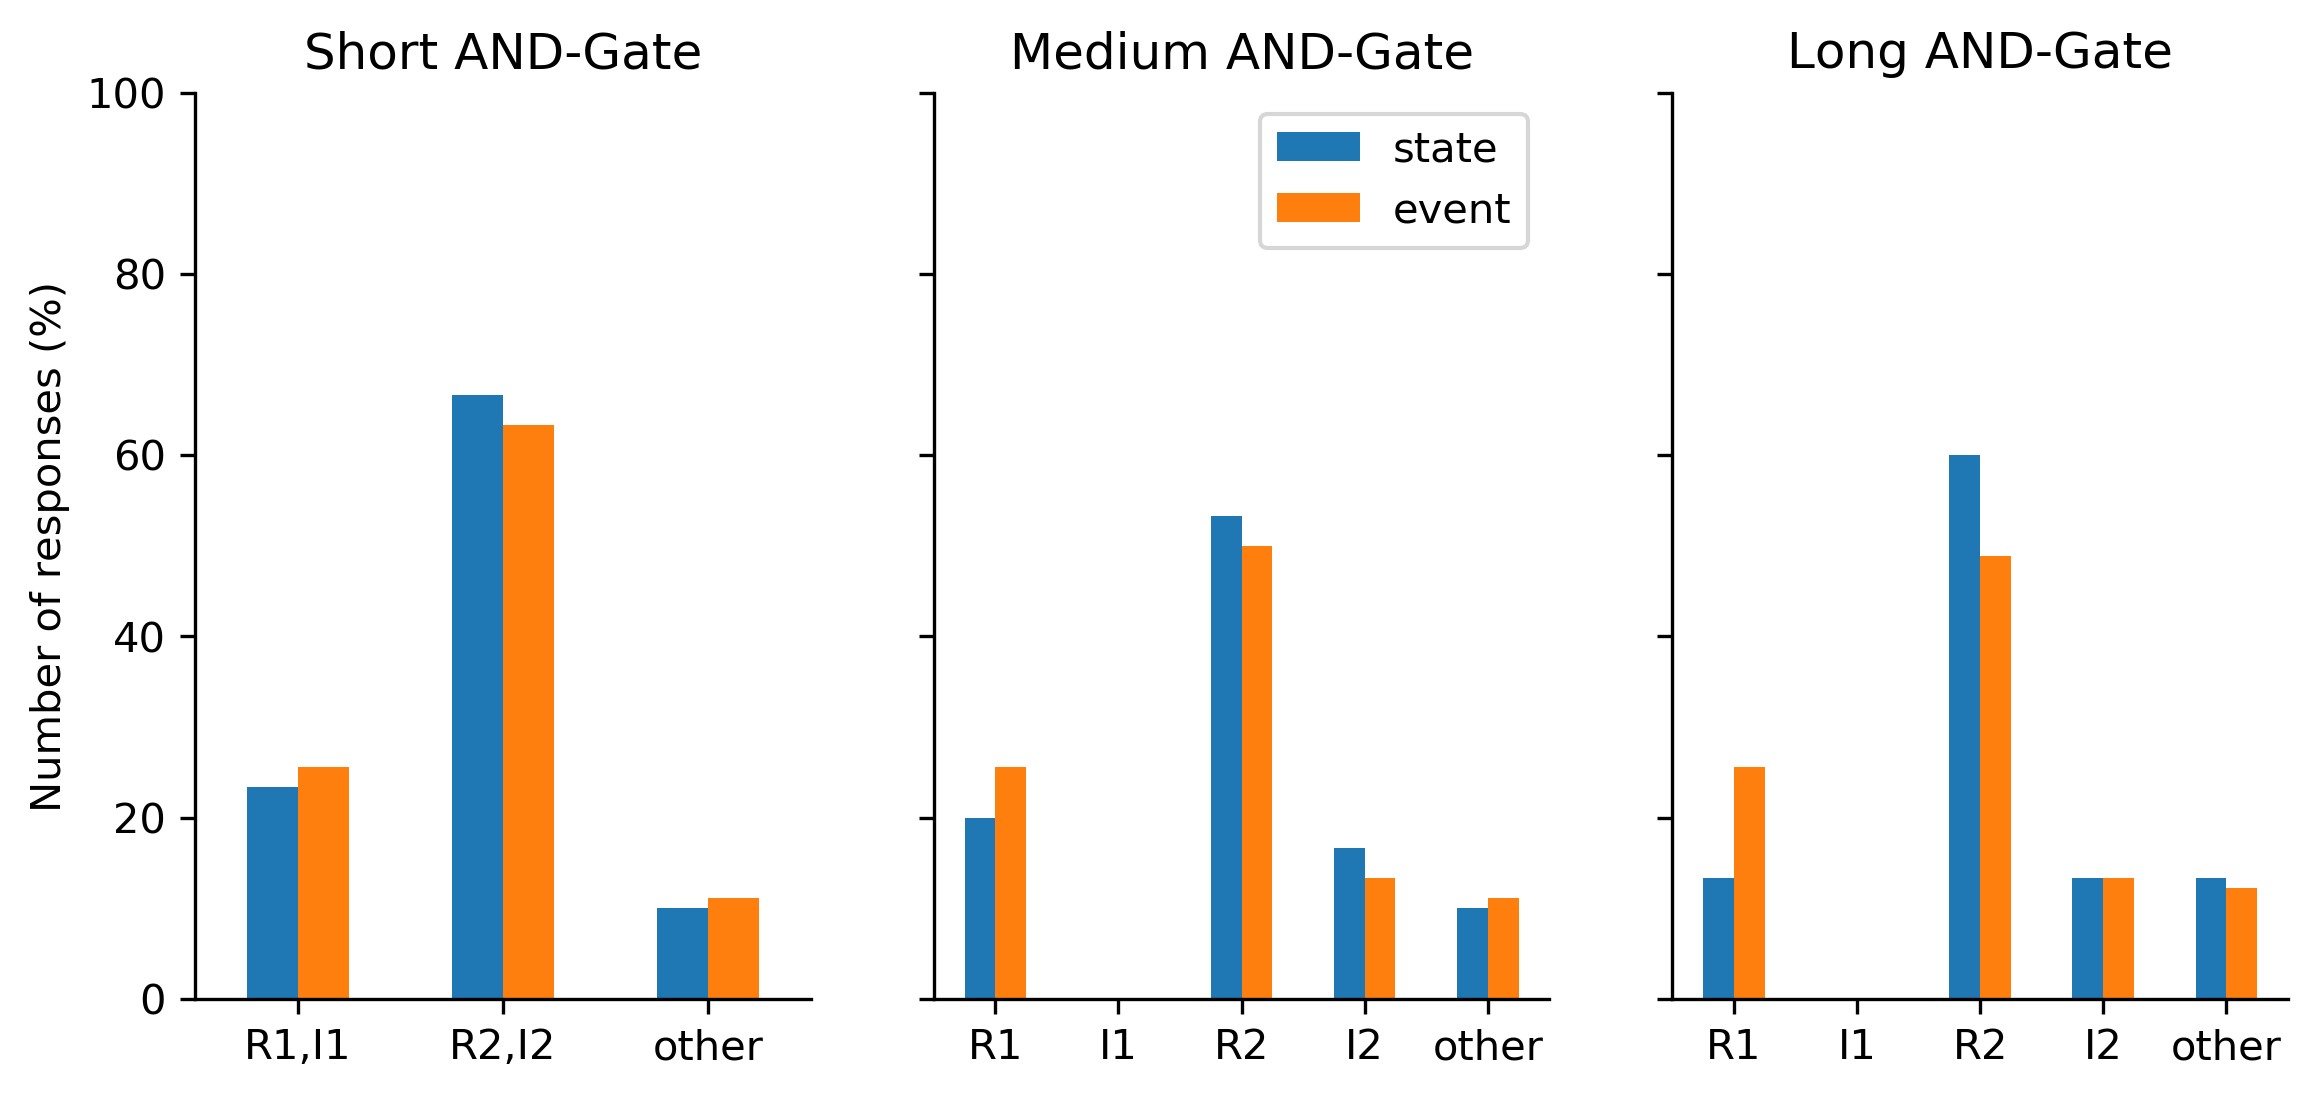
\includegraphics[width=8cm]{results_E1}
\end{center}
\caption{This is a figure.} 
\label{fig:2}
\end{figure}

\textbf{Discussion}. Paragraph...

\subsection{Experiment 2}

\textbf{Participants}. The experiment was hosted by Google App Engine and 89 participants were recruited via Amazon Mechanical Turk. There were 29 females (average age: 39.7), 59 males (average age: 37.6) and 1 declared ``other''. All the participants were english speakers.

\textbf{Method}. Like in Experiment 1 each participant was presented 15 different networks. However this time we introduced round detectors that, contrarily to square detectors, don't maintain their activation through time. By adding this feature we were able to include networks that have a loop of detectors (see Fig.\ref{fig:3b}). 1 stimulus was a chain of square detectors and 1 stimulus was a chain of round detectors were included (for the latter one, only ``G'' remained a square). The other 13 stimuli were AND-Gates and were sorted into three main categories: 4 stimuli were Rolled networks, i.e. with a loop, as depicted in Fig.\ref{fig:3b}, 3 were Unrolled networks with square and round detectors as in Fig.\ref{fig:3a}, labeled ``Unrolled circles'' and 6 stimuli were Unrolled with square detectors in place of the round one (not represented here), labeled ``Unrolled squares''. For each category of AND-Gates all the stimuli were sorted according to two crossed dimensions: ``Event'' \textit{vs} ``State''and ``R1 cont'' \textit{vs} ``R2 cont''. In condition ``Event'' none of the detectors is initially active or -- if the branch is a loop -- is continuously (re-)activated. In condition ``State'' one of the two branches contains initially detectors that are active or is continuously (re-)activated. In condition ``R1 cont'' (represented in Fig.\ref{fig:3a}) the activation is such that there is a continuous sequence of changes going from R1 to I2 that leads to the activation of ``G''. In condition ``R2 cont'' (not represented here) this is R2 that is continously connected to I2 that leads to the activation of ``G''. The design of the experiment for the AND-Gates is given in Tab.\ref{tab:1}. For the AND-Gates (Rolled and Unrolled) the delay between I1 and I2 in condition ``Event'' was maintained at 11 nodes (i.e.1100 ms) for almost all the networks. There was only one Unrolled squares network for which the delay was set at 8 nodes (800ms).

\begin{table}[H]
\begin{center} 
\vskip 0.12in
\begin{tabular}{c|c|c|c|c} 
\hline
\multicolumn{2}{c}{}&\multicolumn{2}{|c|}{Unrolled} & Rolled\\
\cline{3-5}
\multicolumn{2}{c|}{}& Squares    &  Circles & \\
\cline{1-4}
\multirow{2}{*}{Event} & R1 cont & 2 & 1 & 1\\
 & R2 cont & 2 & 1 & 1\\
\hline
\multirow{2}{*}{State} & R1 cont & N/A & N/A & 1\\
 & R2 cont & 2 & 1 & 1\\
\hline
\end{tabular} 
\end{center}
\caption{}
\label{tab:1}
\end{table}

As in Experiment 1 participants were first presented the network in its initial state and were asked to click the ``Run'' button to observe an activation sequence over the network. Participants waited 5000ms to see a first change of state occurring in a detector, except for the Rolled network case with activation already going around the loop (state condition) -- in this case they had to wait between 3800ms and 5700ms before activation starts in the other branch. Activation delay between any two successive squares was set on 100ms as well. 

\begin{figure}[ht]
  \centering
  \subfloat[Unrolled circles.]{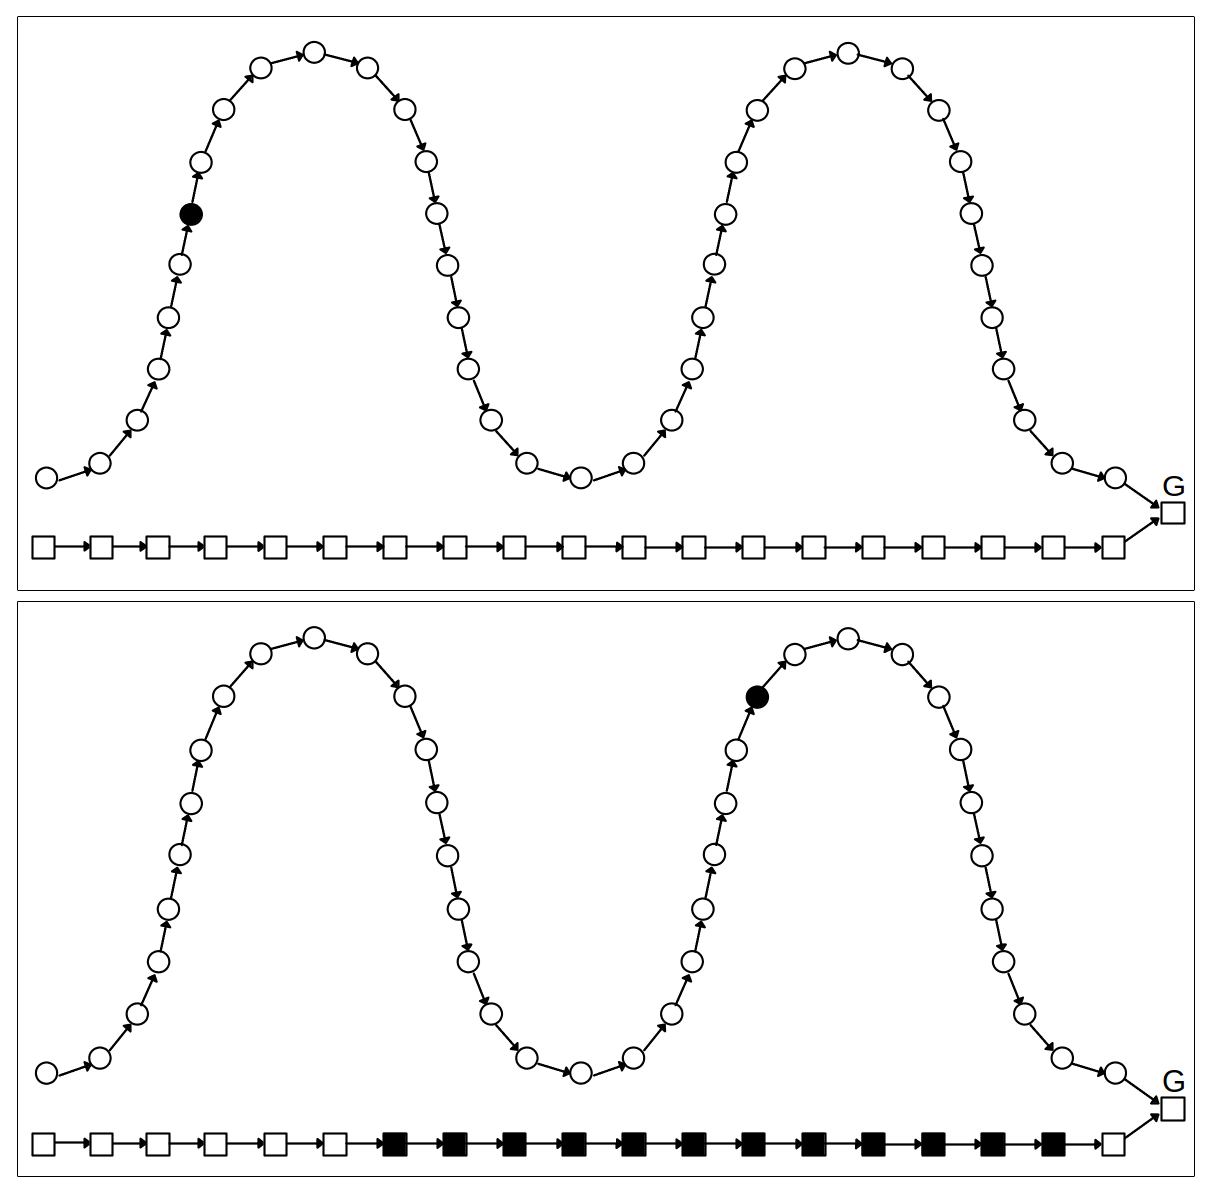
\includegraphics[width=4.2cm]{stim_E2a}\label{fig:3a}}
  \hfill
  \subfloat[Rolled.]{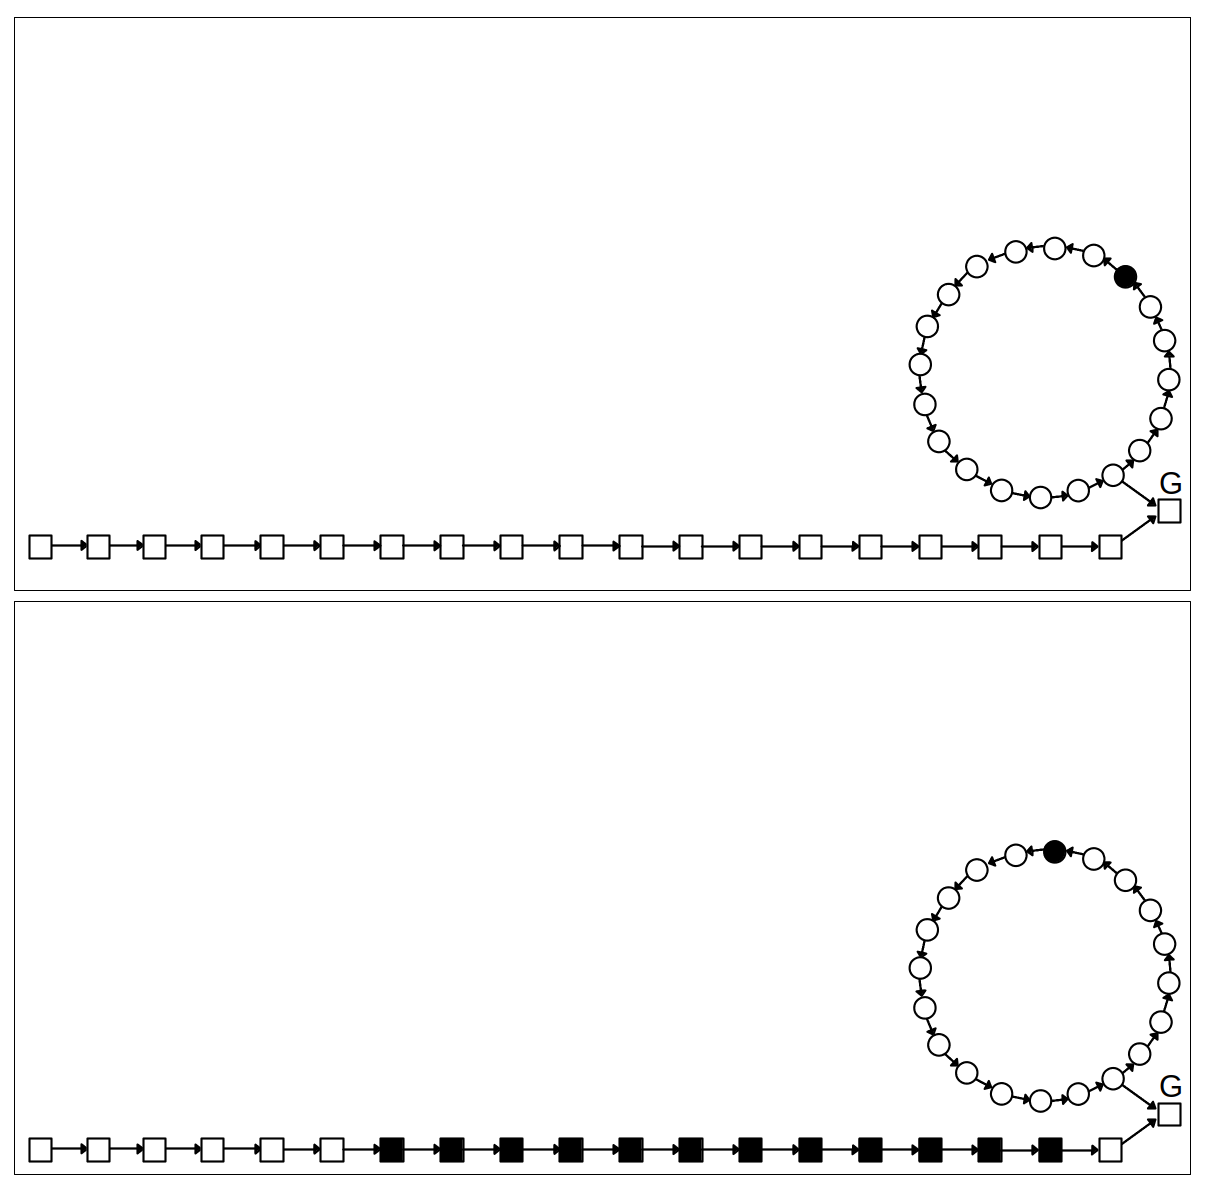
\includegraphics[width=4.2cm]{stim_E2b}\label{fig:3b}}
  \caption{Networks.}
\end{figure}


\textbf{Results}. Paragraph...

\begin{figure}[h]
\begin{center}
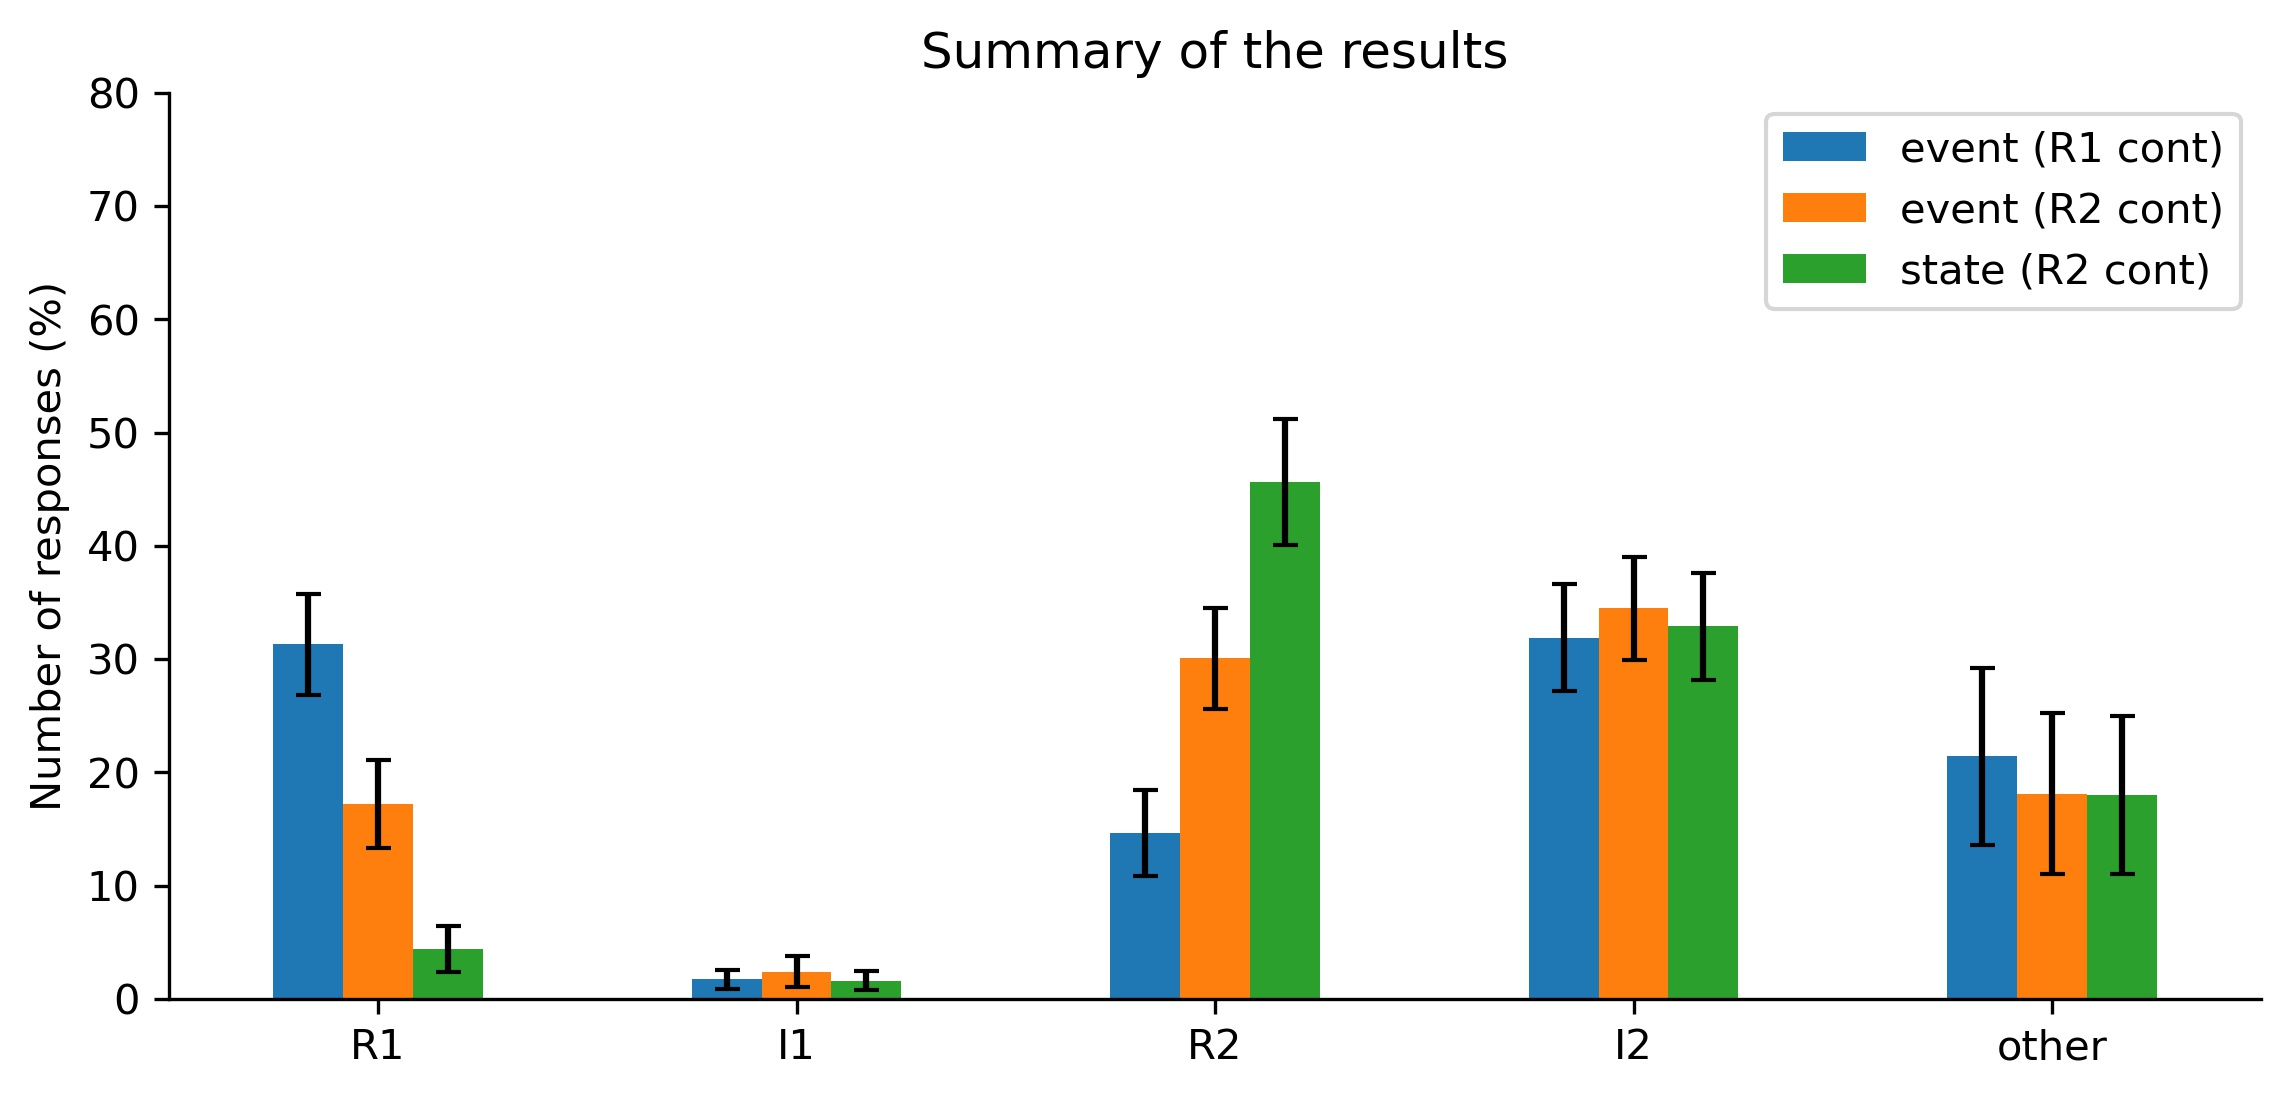
\includegraphics[width=8cm]{results_E2}
\end{center}
\caption{This is a figure.} 
\label{fig:4}
\end{figure}

\textbf{Discussion}. Paragraph...


\section{General discussion}


\bibliographystyle{apacite}

\setlength{\bibleftmargin}{.125in}
\setlength{\bibindent}{-\bibleftmargin}

\bibliography{CogSci_Template}


\end{document}
